\documentclass{article} 
\usepackage[estonian]{babel}
%\usepackage{fontspec} 
\usepackage{graphicx}
\usepackage{hyperref}
\usepackage{natbib}
\usepackage{booktabs}
\usepackage{makeidx}
\usepackage{tgpagella}
\usepackage[T1]{fontenc}
\usepackage{amsmath}
\usepackage{eurosym}

\hypersetup{
    colorlinks=true,       % false: boxed links; true: colored links
    linkcolor=black,          % color of internal links
    citecolor=black,        % color of links to bibliography
    filecolor=magenta,      % color of file links
    urlcolor=black           % color of external links
}

\renewcommand\refname{Viited}

\makeatletter 
\def\s@btitle{\relax} 
\def\subtitle#1{\gdef\s@btitle{#1}} 
\def\@maketitle{% 
  \newpage 
  \null 
  \vskip 2em% 
  \begin{center}% 
  \let \footnote \thanks 
    {\LARGE \@title \par}% 
                \if\s@btitle\relax 
                \else\typeout{[subtitle]}% 
                        \vskip .5pc 
                        \begin{large}% 
                                \textsl{\s@btitle}% 
                                \par 
                        \end{large}% 
                \fi 
    \vskip 1.5em% 
    {\large 
      \lineskip .5em% 
      \begin{tabular}[t]{c}% 
        \@author 
      \end{tabular}\par}% 
    \vskip 1em% 
    {\large \@date}% \\
    \vfill
  \end{center}% 
  \par 
  \vskip 1.5em} 
\makeatother 


\title{IFI7013. IT strateegiline juhtimine}
\subtitle{Märkmed ja kommentaarid}
\date{\today}
\author{Andres Kütt}
%\institute{Riigi Infosüsteemi Amet}

\newcounter{slidenum}
\setcounter{slidenum}{2} % set to 2 if want to exclude title page of presentation

\newcommand\showslide{
%  \clearpage 
  \begin{center}
    \framebox{\includegraphics[page=\arabic{slidenum},width=.99\textwidth]{esimene_kontakt_beamer.pdf}}
%	\includegraphics[page=\arabic{slidenum},width=.65\textwidth]{esimene_kontakt_beamer.pdf}
    \stepcounter{slidenum}
  \end{center}
  \clearpage
}

\begin{document}
\maketitle
\clearpage
\tableofcontents
\clearpage


\section{Arhitektuur}
\subsection{Printsiipidest}
Arhitektuuriga süvitsi tegelemisel on hea mõte pidada printsiipide päevikut. Arhitektuuris on mõttemudelil oluline koht ja seega on mõistlik tegeleda oma isikliku mõttemudeli arendamise ning dokumenteerimisega. Printsiibipäevik on üks viis seda teha. Printsiip on miski, mis tundub kehtivat alati ning mis ei sõltu teistest. Teatavas mõttes on tegemist universaalse tõega. Üheks näiteks printsiipidest arvutivõrkude vallas on \cite{callon1996rfc}. Printsiibipäeviku mõte on selles, et iga kord, kui igapäevases töös tundub mõni printsiip silma jäävat, kirjutatakse see jalamaid üles. Perioodiliselt vaadatakse päevik üle lootuses destilleerida kirja pandust veel universaalsemaid ja üldisemaid põhimõtteid. Üks näide sellisest päevikust on \cite{archprinciples}. 

\subsection{Emergentsusest}
Ingliskeelsel terminil \emph{emergence} on eesti keeles vasteks emergentsus. Nii tähistatakse süsteemi omadust, mis seisneb millegi ilmnemises tänu mingitele muudele süsteemi omadustele. Arhitektuuri kontekstis on emergentsus süsteemide omadus lisaks disaini kaudu eesmärgiks seatud omadustele ka teiste omaduste ilmnemiseks. Tüüpiline emergentne omadus on võime inimesi tappa: suur hulk tehnoloogiaid alates tulest ja lõpetades tuumareaktsiooniga on mingil hetkel osutunud efektiivseks vaenlastest vabanemise vahendiks. Esimene nuga ei olnud mõledud mõrvaks kuid seda on nii aegade algusest kasutatud. Tüüpiliselt ei ole probleem mitte niivõrd süsteemi enda emergentsed omadused vaid emergents, mis sünnib eri objektide kombinatsioonist. Laua funktsioon on toetada asju. Joonlaua funktsioon on sirgeid jooni tõmmata. Kui aga asetada joonlaud poolenisti lauale, oleme saanud, sõltuvalt vaatepunktist, kas muusikariista või inimeste ärritamise vahendi. 

Mitte kõik emergentsed omadused ei ole lihtsalt ebasoovitavad või ootamatud \cite{emergence} toob häid näiteid sellest, kuidas pilvelõhkujad oma arhitektuuriga lausa inimesi ohustada võivad.

\subsection{Süsteemi piiride probleem}
Kui rääkida süsteemist, tekib alati küsimus süsteemi piiridest: kus algab meie kontrolli all olev ala ja kus ta lõpeb? \cite{wood2013framework} räägib osapoolte kaasamisest ning probleemipüstituse juures küsib õigesti: kuidas saada kontrolli alla konkreetse rakenduse teise ja kolmanda järgu efektid? Ehk, kuidas vältida projekti ebaõnnestumist, sest temast tõusis kahju meie olulise kliendi olulisele partnerile? Lahendusteks pakutakse osapoolte omavaheliste suhete analüüsi sotsiaalvõrkude puhul kasutatavate meetoditega. Siiski ei anta ka siin vastust küsimusele kirjeldatud võrgu piiridest: ei ole selge, kuidas otsustatakse, keda võrku kaasata ja keda mitte (kas kliendi kliendi klient on ka oluline?). 

Lisaks konkreetsele osapoolte kaardistamise raamistikule annab artikkel ka mõningase ülevaate erinevatest EA raamistikest.

\section{Äriplaan}
\subsection{Arendus- ja halduskuludest}
\label{sec:kulud}
Laias laastus võib öelda, et kulud arendusele jagunevad kuludeks, mis tarnivad uut funktsionaalsust (ning mida tavaliselt tajutakse kui uut väärtust lisavatena) ning kuludeks, mis lähevad olemasoleva muutmiseks või parandamiseks. Neist esimesed lisavad selgesti halduskoormust ja halduskulusid luues uusi rakendusi, mida tuleb hallata, millede teenustase tuleb tagada. Teised aga võivad (aga ei pruugi) halduskulusid vähendada näiteks tehnilist tehnilist võlga likvideerides. Arenduskulusid võib vaadata ka keerukuse vaatepunktist: esimest liiki kulud suurendavad, teised võivad aga keerukust vähendada. Kokkuvõte kuludest ja nende mõjudest on toodud tabelis \ref{tab:arendus}.

\begin{table}
	\begin{center}
		\begin{tabular}{p{3.8cm}p{2.4cm}p{2.1cm}p{2.7cm}}
		\toprule
Kulu & Mõju \mbox{halduskuludele} & Mõju tajutud väärtusele & Mõju \mbox{keerukusele} \\
\midrule

Uue funktsionaaluse \mbox{lisamine} & Selgesti \mbox{suurendab} & Selgesti \mbox{suurendab} & Selgesti \mbox{suurendab} \\
\addlinespace
Olemasoleva muutmine või parandamine & Neutraalne või vähendab & Reeglina \mbox{neutraalne} & Neutraalne, \mbox{pigem} vähendab \\

\bottomrule
		\end{tabular}
		\caption{Kokkuvõte arenduskulude mõjust}
		\label{tab:arendus}
	\end{center}
\end{table}

Siit tuleneb oluline tõdemus: arenduskulud, mis suurendavad tajutud väärtust tekitavad juurde ka halduskoormust ja lisavad keerukust viies seega alla organisatsiooni võime tulevikus uut väärtust lisada. Võtmeks tupikust välja on sõna "tautud". Muutes viisi, kuidas organisatsioon tajub ITst tulenevat väärtust on võiamlik saavutada tellija arusaam IT kulude dünaamikast. 

\subsection{Arhitektuur ja äri}
Toote või teenuse arhitektuur mõjutab otseselt orgranisatsiooni ärilist positsiooni. Vaatleme neid seoseid Crawley arhitektuurimudeli taustal (joonis \ref{fig:arh}). Nagu loengus räägitud, on arhitektuuril kolm olulist komponenti: vorm, funktsioon ja kontseptsioon. Vorm on see, mis "on", funktsioon on see, mida tehakse ning kontseptsioon seob need tervikuks. Toote või teenuse väärtus tuleneb tema funktsioonist: mida täpsemalt vajadust täidetakse ning mida põletavam too vajadus, seda väärtuslikum toode või teenus. Süsteemi kulud tulenevad aga kogu elutsükli jooksul vormist: selleks tuleb hankida materialid, viia läbi tootmine ning lõpuks utiliseerimine. Järelikult tuleneb vormi ja funktsiooni vahekorrast (mida suuresti määratleb kontseptsioon), organisatsiooni võimekus kasumit teenida.

\begin{figure}[htp]
	\begin{center}
		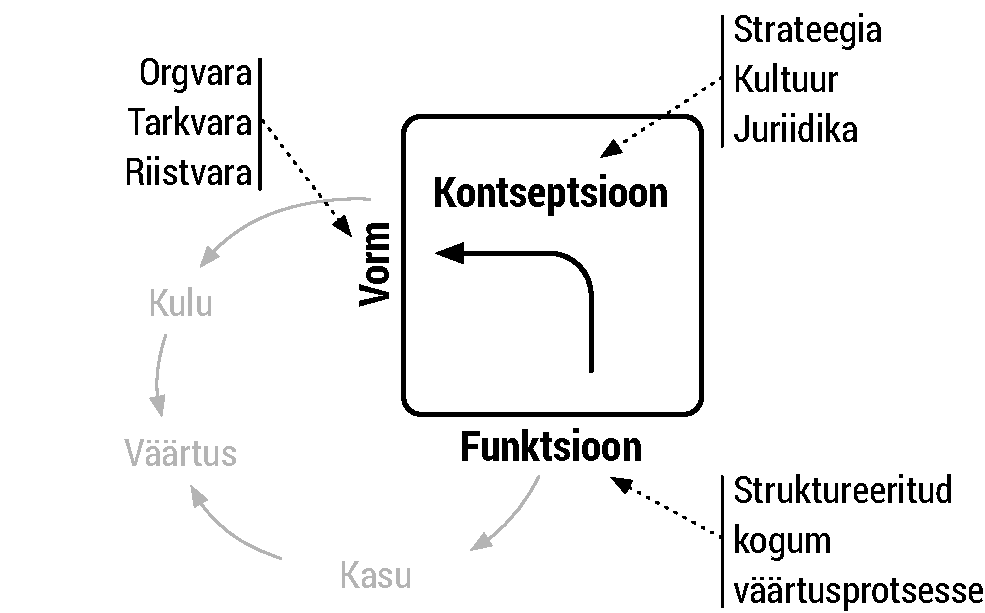
\includegraphics[width=.6\textwidth]{ffc_profit.pdf}
		\caption{Organisatsiooni finantside seos arhitektuuriga}
		\label{fig:arh}
	\end{center}
\end{figure}


On oluline mõista, et hea arhitektuur ei ole kasumiks piisav vaid pelgalt tarvilik: lisaks arhitektuurile on vaja veel paljut alates näiteks korralikust turundusest kuid ilma arhitektuurita ei ole kasum mõeldav. 

Kasumi ja arhitektuuri seoseid illustreerivaid näiteid on nii kaugemast kui lähemast minevikust mitmeid. Positiivsena tasub esile tuua Black \& Deckeri strateegilist tooteinnovatsiooni seitsmekümnendatel ning Volkswageni platvormistrateegiat. Negatiivsena on üks tuntumaid General Motorsi lähenemine platvormidele. 


\section{Tarkvaratehnika}
\subsection{Kokkuhoiust programmeerijatelt}
\label{sec:kokkuhoid}
Joel ütleb õigesti, et programmeerijate arendamiselt kokku hoida ei ole mõistlik. Sama kehtib ka teiste valdkondade inimeste puhul, kuid programmerijate töö on teiste omast suhteliselt info- ja teadmismahukam.

Valest kohast kokku hoitud raha (või värbamisel tehtud vead) võivad viia järgmise tagasisideni (vt. joonis \ref{fig:kokkuhoid}\footnote{Pluss-märk noolel ei tähenda mitte positiivset mõju vaid seda, et muutujad liiguvad samas suunas: ühe tõusule järgneb teise tõus ja langusele langus}):
\begin{enumerate}
	\item Koodi kvaliteet on madal
	\item Mistõttu kulub suhteliselt rohkem raha vigadega tegelemiseks ja teenitakse vähem
	\item Mis viib alla ettevõtte võimekuse inimestesse investeerida
	\item Mispeale langeb inimeste kompetentsitase veelgi (tehnoloogia ju areneb)
	\item Madalad kompetentsid viivad aga madalale koodi kvaliteedi
\end{enumerate}

Eesti IT-ettevõtted jagunevad ITLi andmetel suhteliselt radikaalselt kaheks: suured ning kasumlikud ning väikesed ja virelevad. Seda veelahet võib seletada läbi selle, kellel on õnnestunud tsükkel mis pidi tööle panna sest, muidugi, kehtib ka vastupidine. Kõrge koodi kvaliteet viib suuremate sissetulekuteni jne.

\begin{figure}[htp]
	\begin{center}
		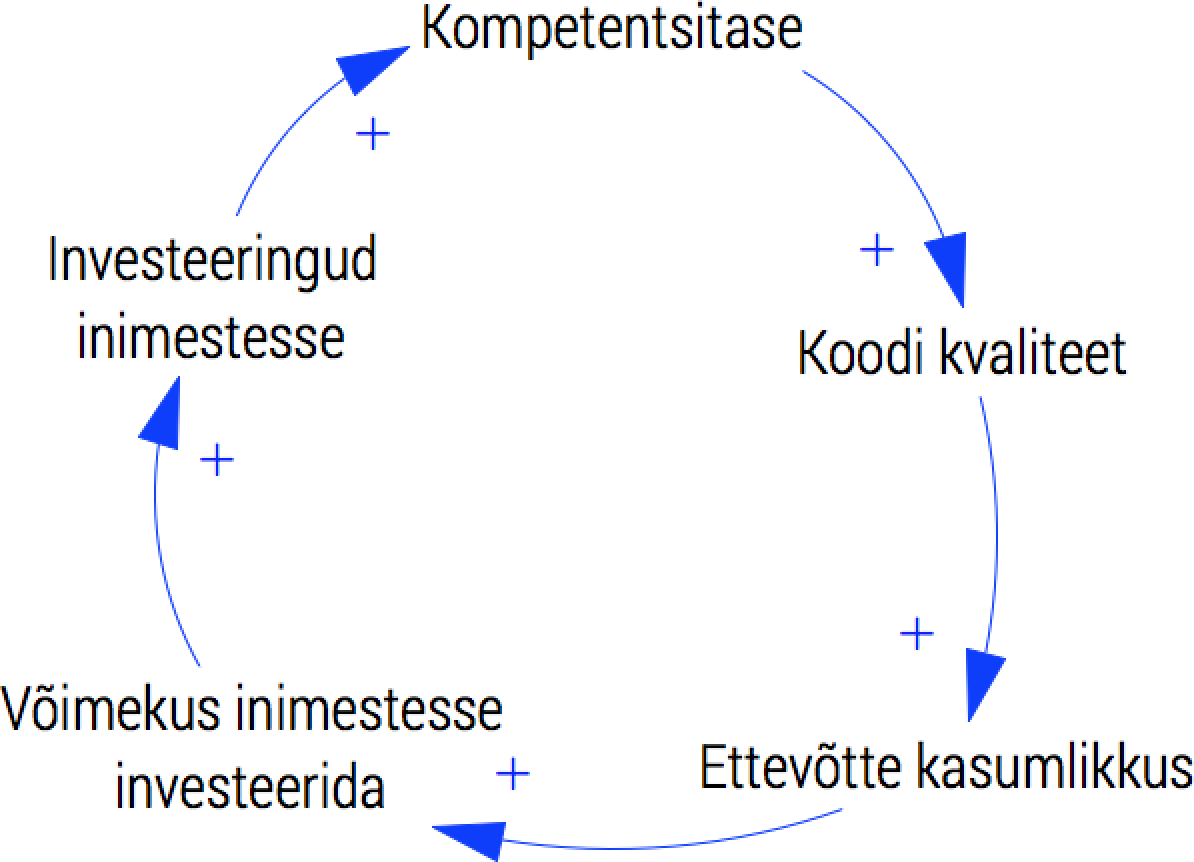
\includegraphics[width=.6\textwidth]{kvaliteet.png}
		\caption{Kokkuhoiu tagajärjed}
		\label{fig:kokkuhoid}
	\end{center}
\end{figure}

\subsection{Kood ei roosteta. Või siiski?}
\label{sec:rooste}
Joel Spolsky ütleb, et reeglina on väga halb mõte oma koodibaasi ümber kirjutada, sest kood ju "ei roosteta" \citep{joelrust}. Ta toob mitu näidet väga ebameeldivate tagajärgedega ümber-kirjutamis ettevõtmiste kohta ning, tõesti, neid on ka siinkirjutaja praktikas mitmeid ette tulnud. Põhjuseid on mitmeid, peamiseks ehk paratamatu teadmuskadu: iga tükki koodi on juba enne rakenduse valmimist kümneid kui mitte sadu kordi muudetud ja parandatud parandamaks vigu, ületamaks nõuete ebatäielikkust jne. Nii kaob igasugune võimalus hinnata, kas kood on selline, nagu ta on, põhjusega või põhjuseta. Rääkimata analüüsist, kas põhjus jätkuvalt kehtib. Miks siis tekib vahel siiski kohu asju ümber teha ning miks on Eestis kehtestatud \emph{no legacy policy}?

Ühest küljest on asja taga kindlasti programmeerijad. Nagu Spolsky õigesti osundab, on koodi lugemine palju keerulisem, kui selle kirjutamine. Seega, eriti kui tegu on kellegi teise koodiga, on programmeerijale oluliselt lihtsam kirjutada uus kood kui üritada vanast aru saada. Loomulikult tõlgitakse vahe rahanumbriks ning uue süsteemi ehitamine võib vana turgutamisest oluliselt odavam näida. Erinevalt uue süsteemi ehitamisest, ei ole vana muutmine kergesti hinnatav ning tellija ees on kas väike fikseeritud number ebamäärase kahjuga või suur riskantne number ebamäärase tuluga. 

Teisalt võib ümberkirjutamissoovi taga olla lihtne äriliste riskide vähendamine. Vana kood peidab endas alati üllatusi ning riskide vähendamiseks võib pakkuja eelistada uue kirjutamist. 

Mõlemal juhul tekib lihtsasti olukord, kus tellijal ja otsuse tegijal ei ole piisavalt tehnilist teadmist ja/või informatsiooni vana süsteemi kohta. Erinevalt koodist teadmus kindlasti kõduneb. Sel puhul on mõistlik käivitada väikesemahuline konkreetsete tulemustega piloot rakenduse kvaliteedi hindamiseks. Selle lõppedes on nii tellijal kui täitjal palju selgem ülevaade, kui keeruline vana koodibaasi putitamine tegelikult on.

Olemasoleva koodi puhul võib tegu olla ka "pusaga": süsteemiga, mis on aja jooksul kas arhitektuuriliselt või tehnoloogiliselt keeruliseks kasvanud. Nii arhitektuuri kui tehnoloogia puhul on kindlasti tegu ka mööduva moega, tehno\-loogiad ning arhitektuurimustrid vananevad. Samas ei ole kindlasti tegu \textit{carte blanche} põhjusega rakendusi ümber kirjutada, COBOLi süsteeme on edukalt veebirakendustega integreeritud. Jällegi on mõistlik läbi viia piloot ning teha otsus kindla teadmise, mitte kellegi arvamuse pinnalt.

\begin{figure}[htp]
	\begin{center}
		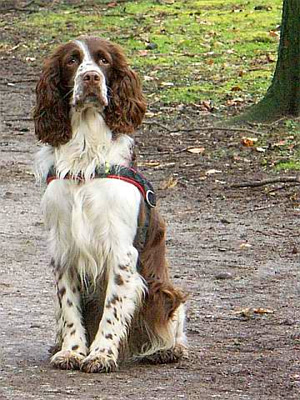
\includegraphics[height=4cm]{spaniel.jpg}
\includegraphics[height=4cm]{wolf.jpg}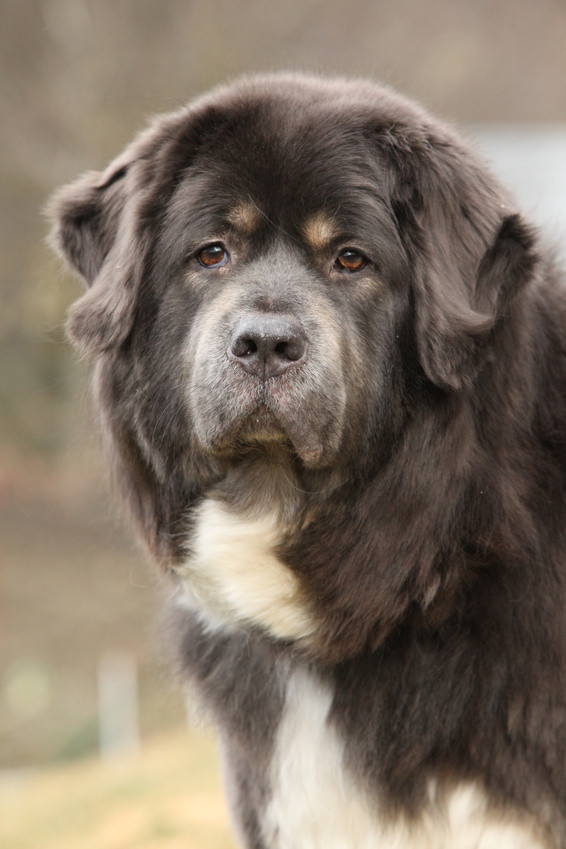
\includegraphics[height=4cm]{mastiff.jpg}
		\caption{Spanjel, hunt ja mastif}
	\end{center}
\end{figure}

Niisiis, koodi ümber kirjutamine on kallis, keeruline ning seotud oluliste riskidega. Samas on olemasoleva rakenduse putitamisel samuti üks oluline puudus: me toimime jätkuvalt kord juba defineeritud arhitektuuri, täpsemalt öeldes kontseptsiooni, raamides. Ehk, asjade ümber kirjutamine annab võimaluse innovatsiooniks ning asjade puhtalt lehelt uuesti mõtestamiseks. Jah, spanjelist on ilmselt võimalik mastifi-laadne elukas aretada aga võibolla on efektiivsem alustada siiski nende ühisest eellasest, hundist? Kindlasti tuleks keskenduda mitte tehnilisele vaid ärilisele innovatsioonile ümber mõtestades äriprotsesse, automatiseerides ning efektiivistades. Seejuures on muidugi eelduseks, et meil on piisavalt aega ja raha seda mõttetööd põhjalikult ette võtta ning et on alust eeldada, et tulemus praegusest olukorrast oluliselt erineb.

Lõpuks tuleb panna kõrvuti süsteemi ümber kirjutamise kulu (korrutades esiaglse hinnangu vähemalt kahega), olemasoleva muutmise ning mõlema alternatiivi halduskulude nüüdisväärtus. Kui nüüd tundub, et rakenduse uuesti kirjutamine on siiski mõistlik, on oluline aru saada, miks nii läks. Jällegi Joelile toetudes, ei ole mõistlik eeldada, et kui ühel korral ei õnnestunud hankida mõistlikku süsteemi või seda pusaks muutumast hoida, siis teisel korral asjad teisiti lähevad. On oluline, et suudetakse välja tuua konkreetsed tegevused, mille abil hoidutakse vajadusest süsteem uuesti ümber kirjutada. Siinkohal kuuleb ilmselt argumenti \emph{build one to throw away} aga sel juhul peaks olema võimalik vähemalt üles kirjutada, mida esimesest korrast täpselt õpiti.

\subsection{Tehniline võlg}
On kriitiline, et tellija saaks aru oma tegevuse tagajärgedest. Mis, arvestades teo ja selle tagajärje ajalist vahet, on väga keeruline. Põhjus on selles, et tehnilise võla likvideerimine tuleb arenduse läbilaskevõime arvelt. Järelikult tähendab tehnilise võla kuhjumine, et arenduse läbilaskevõime ajas kahaneb. Kui tellija ei saa aru, et tema otsus tekitas tehnilise võla, on IT-juhil kaks põhimõttelist otsust. Ta kas keeldub tehnilist võlga tekitamast, näib paindumatu ja lastakse lahti või ta võtab tehnilise võla, asub seda IT võimekust vähendades likvideerima ning ta lastakse lahti. Ehk, häid valikuid ei ole. Järelikult ei ole IT juhil muud valikut peale tellija harimise.

Tehnilise võla oluline aspekt on seotud süsteemi piiride küsimusega. Kuna tehniline võlg on seotud konkreetse süsteemiga kuid, definitsiooni järgi, on süsteemi piirid alati suvalised, võib rääkida tehnilise võla skoobist. On võimalik olukord, kus lokaalsete optimumide saavutamise läbi võetakse süsteemi kui terviku suhtes tehnilist võlga. Näiteks võib ehitada kõik süsteemid tähtajaks kuid mitte arvestades teiste süsteemi osade integratsioonivajadusi. Üksiku süsteemi vaatepunktist võlga ei ole. Süsteem kui tervik aga võib vajada olulist investeeringut oma komponentide suhtluse tagamiseks. 

Tehnilise võla juhtimine on teatavas mõttes sarnane finantsvõla juhtimisega: rahavoogude nüüdisväärtuse abil on võimalik teha otsuseid. Tehnilisel võlal on siiski ka aspekte, mida lihtsasti finantsmudelisse valada ei õnnestu. Teatavast piirist alates hakkab tehniline võlg takistama värbamist ja inimeste hoidmist. Tegemist on raskestivarjatava stressifaktoriga ning üha vähem leidub inimesi, kes "selle supiga" on nõus tegelema. Nii võib alata lõigus \ref{sec:kokkuhoid} kirjeldatuga sarnane tagasiside, kus kompetentsete inimeste lahkumine viib võla suurenemiseni mis omakorda tõrjub kompetentseid inimesi. 

\section{IT valitsemine}
\subsection{Poliitikavastasus. Hundid ja jänesed}
Kujutlegem lihtsat ökosüsteemi, mis koosneb huntidest ja jänestest. Hundid söövad jäneseid, jänesed elavad õhust ja armastusest (mida mõlemat on piisavalt). Oletagem, et meil on soov tõsta huntide arvukust. Seepärast tuuakse mujalt ja lastakse metsa lahti viis emast ja viis isast hunti. Mis juhtub? 
\begin{itemize}
	\item Huntide arvukus tõuseb kümne lisandunud hundi võrra
	\item Kuna kümme lisandunud hunti tahavad süüa, siis väheneb jäneste arvukus. Ajaühikus ära söödavate jäneste hulk ju suureneb
	\item Kuna jäneseid on vähem, väheneb ka jäneste juurdekasvu kiirus. Ära söödud jänesed ju uusi jäneseid ei tee. Samuti tahavad uued hundid ka homme süüa
	\item Seega hakkab jäneste arvukus vähenema
	\item Misjärel hakkavad hundid nälga jääma, sest kõigile enam jäneseid ei jagu
	\item Mistõttu saavad hundid vähem järglasi ja langeb nende juurdekasvu kiirus
	\item Kuna hundid surevad vanadusse ikka sama tempoga, hakkab huntide arvukus vähenema
	\item Kui huntide arvukus on jõudnud esialgsele tasemele, on kõigile jälle piisavalt jäneseid 
\end{itemize}

Nii taastub esialgne olukord, algne huntide lisamine ei ole andnud soovitud tulemust. Huntide arvukus võiks tõusta hoopis tõstes jäneselaste arvu jäneseperekonnas ehk nende juurdekasvu kiiruse tõstmisega. 

\subsection{Inimeste valitsemine}
Valitsemise üsna lahutamatu osa on paraku vajadus inimesed organisatsioonist eemaldada. Jättes kõrvale juriidilised ja muud nüansid, on oluline aru saada, et mõtteliidri (\emph{thought leader}) lahkumine on meeskonna dünaamika jaoks oluline sündmus. Samuti on oluline mõista, et tegu on vältimatu protsessiga, mis seega on mõistlik läbi viia kontrollitult ja minimaalsete kadudega. Järgnevas selleks mõned näpunäited: 

\begin{itemize}
	\item Vii inimene organisatsioonist välja enne, kui tema vastuolud muutuvad meeskonna vastuoluks. Definistiooni järgi inimesed järgnevad liidrile ning kui tollel on kellegagi vastuolud, kanduvad nood paratamatult varem või hiljem meeskonda. Kui hiljaks jääda lahkuvad (või tuleb vastuseisu tõttu eemaldada) ka teised tiimi liikmed peale juhi. Nii võib oskamatu käitumisega vallandada lumepalliefekti, mis organisatsiooni kiiresti ajudest tühjendab.
	\item Väike (!) hulk võtmeisikuid peab plaanist ette teadma, sealhulgas muidugi ka eemaldatav ise. Nii on neil ühest küljest võimalik tulevaseks kriisiks valmistuda kuid teisalt saab nii vältida emotsionaalset avalikku käitumist ning muidu üllatusi. Etteteatamisaeg võib ulatuda mõnest päevast mõne tunnini. Pikem aeg tekitab permanentse kriisi olukorra ja kommunikatsioon väljub kontrolli alt
	\item Kommunikatsiooni kolm sammu. Kõik sammud läbitakse väga lühikeste (kõige rohkem mõned tunnid) intervallidega vältimaks uudiste lekkimist (ingl. \emph{techcrunch meltdown} tuntud tehnoloogiauudiste portalli järgi) ning minimeerimaks kriisi kestvust. 
		\begin{enumerate}
			\item "Vanaisa"\footnote{Juhi juht. Selles kontekstis isik, kes teeb otsuse inimene välja viia.} teade. Nii antakse teada, kes olukorda kontrollib. Sisaldab
				\begin{itemize}
					\item Kes lahkub millal ja miks. Tekst olgu viisakas, inimesed kas teavad niigi või suudavad ridade vahelt lugeda
					\item Mis juhtub järgmisena ja millal. Inimestele ei meeldi ebakindlus, hirmud tuleb maha võtta. Oluline punkt siin: kes ja millal asendab lahkuja?
					\item Muutused organisatsiooni toimimises. Lahkuja oli kindlasti osaline mingites äriprotsessides (koodi ülevaatused, tarnete vastu võtmine jms.), kuidas need edasi toimima hakkavad?
				\end{itemize}
			\item Lahkuja teade. Tavaliselt suunatud lähematele kolleegidele. Võib olla suhteliselt otsekohene aga kui on karta midagi mürgist, võib (viisakalt) paluda teksti kooskõlastamist
			\item Avalik teade. Kui vähegi usutav, võiks tekst olla kiitvas, positiivses ja tänulikus toonis. Kui mitte, siis lakooniline kuiv tekst.
		\end{enumerate}
\end{itemize}

\subsection{Ressursijuhtimine}
Järgnev on üks võimalik vaade asjadele: selgesti on avaliku- ja erasektori suhtumine rahasse erinev. Ainus põhjus, miks maksumaksja riigile raha annab, on, et selle raha eest osutataks avalikku teenust. Kui nüüd riik korjab raha kokku, kuid selle eest mõistlikku avalikku teenust ei osuta (ka reservide kogumine on avalik teenus), siis on tegu maksumaksja asjatu koormamisega. Erasektoris jaotatakse kasum omanike vahel, riigis selle mehhanismi ekvivalenti ei eksisteeri. Järelikult on erasektoris pigem surve raha mitte kulutada samas kui riigisektoris on pigem surve raha eest võimalikult palju teenust osutada.  

\subsection{Protsesside juhtimine}
\subsubsection{Organisatsiooni kiirendamine}
Suurepärane näide organisatsiooni kiirendamisest on Singapur. Joonisel \ref{fig:kasv} on toodud viie riigi GNI aastatel 1995 kuni 2012. On näha, kuidas USA, Eesti, Läti ja Vene Föderatsioon kasvavavad suuresti samas rütmis, kuigi absoluutnumbrites on USA teistest kaugel ees. Singapur aga on suutnud aastast 2002 näidata teistest oluliselt kiiremat kasvu. Isegi arvestades 2008. aasta kriisi mõju, on kasv teistest oluliselt kiirem. Lühike järeldus joonisest on, et ühel või teisel viisil on Singapur suutnud mitte ainult kasvada, vaid kasvada teistest kiiremini. Kui Eesti aga ka jätkab senist stabiilset kasvu, ei õnnestu meil ilmselt kunagi USAle järele jõuda. 

\begin{figure}[h]
	\begin{center}
		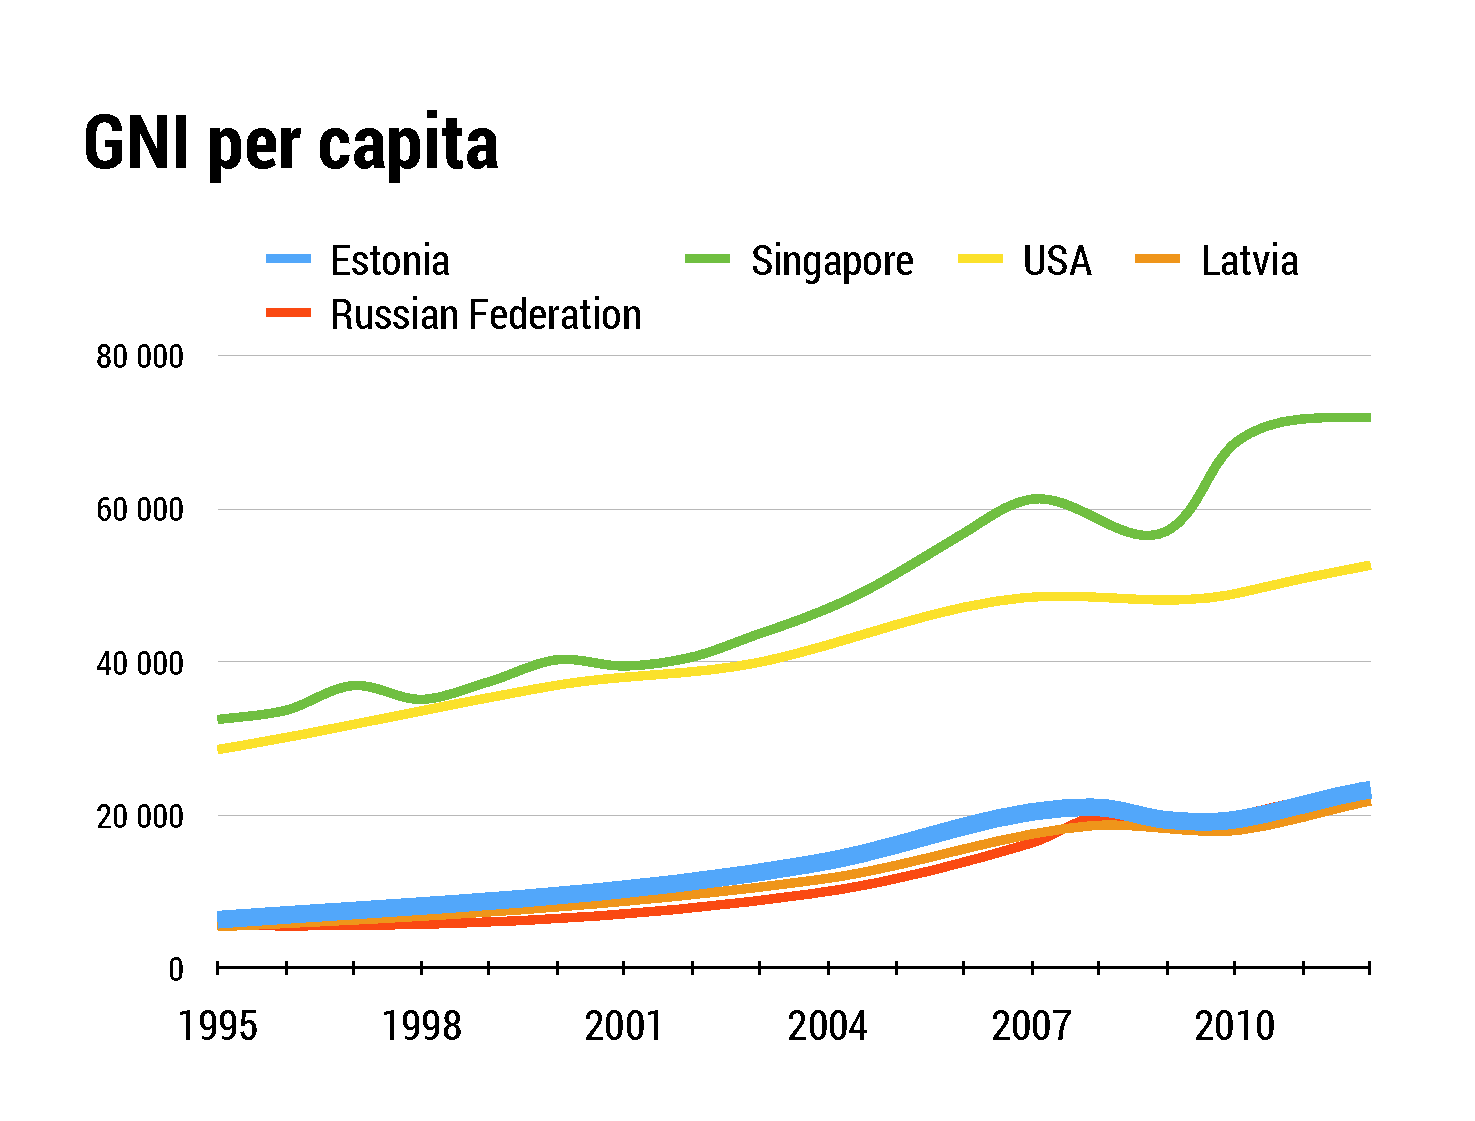
\includegraphics[width=\textwidth]{kasv.pdf}
		\caption{Riikide GNI võrdlus. Maailmapanga andmed.}
		\label{fig:kasv}
	\end{center}
\end{figure}

\subsubsection{Arenduse ootejärjekorra juhtimine}
Infotehnoloogia on tavaliselt põimunud sügavale organisatsiooni protsessidesse. Samuti on IT peamine protsesside efektiivistamise vahend. Järelikult on igas organisatsioonis suur hulk erinevaid arendusvajadusi. Samas on ressursid alati piiratud\footnote{Rangelt võttes võib probleemiks olla ka võimekus ressursside omavaheline vahetus. Näiteks on suurettevõtetes või avalikus sektoris tihti piiratud täistööajaga töötajate hulk, samuti võib saadaolev finantseering olla seotud pirangutega (selle kulutamine teatud riigis või teatud tegevusteks)} ning seega ületab organisatsiooni arendusvajadus reeglina IT-organisatsiooni võimekust seda vajadust täita\footnote{Vt. ka lõik \ref{sec:kulud} organisatsiooni võimekuse arengu kohta}. Järelikult kerkib küsimus tööülesannete järjestamisest. Mis järjekorras töid ette võtta?

Ootejärjekorral on järgnevad omadused:
\begin{itemize}
	\item Kuna töid tekib definitsiooni järgi kiiremini, kui neid täita suudetakse, siis järjekord kasvab. Kui vannist voolab vesi aeglasemalt, kui seda sinna lisandub, hakkab vee tase tõusma
	\item Mida pikem on ootejärjekord, seda paindumatum on organisatsioon. Kui järjekorras on x aasta jagu projekte, siis jõuab järjekorra viimane tegemisse kõige kiiremini x aastaga
	\item Kuna organisatsiooni äritulemuste saavutamine sõltub sageli ITst, eksisteerib ootejärjekorrale tugev poliitiline surve. Otsus mõnda projekti teha ja teist mitte võib omada mõne osalise jaoks omada isiklikku väljundit tulemustasu näol
\end{itemize}

Et ootejärjekord on pikk, tuleb ühel või teisel viisil sealt kas projekte välja jätta või vähendada organisatsiooni võimekust sinna asju lisada. Et otsused on seotud konfliktiga, minnakse sageli just ootejärjekorra barjääri tõstmise teed. Oma rolli mängib siin ka soov olemasolevat võimalikult efektiivselt kasutada suunates klienti võimalikult põhjalikku eeltööd tegema. IT kliendiks oleva keskastme juhi vaatenurgast vaadates tekib nii olukord, kus tema (organisatsiooni perspektiivist väheoluline, kuid tema jaoks kriitiline) arendusvajadus vajab ebaproportsionaalselt palju panust ning omab ikkagi väikest shanssi töösse minna. Eriti drastiline on probleem harukontorite puhul, millede probleemistikust ei pruugi lõpuni aru saada ka peakontori inimesed. Kui nüüd tollel juhil on initsiatiivi, juhtub tavaliselt üks kahest. Kui käepärast on krediitkaart, siis võidakse probleemi lahendamiseks hankida marginaalse hinna eest teenust mõnelt SaaS\footnote{\emph{Software as a Service} tarkvara kui teenus. Lahendus, kus tarkvara hallatakse keskselt ning lõppkasutaja maksab teenuse eest perioodiliselt proportsionaalselt teenuse kasutamisega} pakkujalt. Mispuhul tekib reeglina kohe riskijuhtimislik probleem sest kaob kontroll organisatsiooni andmete üle. Kui aga käepärast on IT-kompetentsi kas Exceli makrode või PHP tundja näol, luuakse tõenäoliselt kohalik infosüsteem. Sedalaadi infosüsteem ei vasta tavaliselt ühelegi keskse IT standardile, muutub ühel hetkel tellija jaoks kriitiliseks, kaotab oma ainsa arendaja (vahel kõike korraga) ning paneb keskse IT fakti ette: üle tuleb võtta dokumenteerimata, ebaturvaline ja profiilist välja jääv ärikriitiline tehniline lahendus. Tekitatud pusa ümber kirjutamiseks (kui isegi leidub keegi, kes suudaks sellise ülesande pädevalt püstitada) reeglina finantseeringut leida ei õnnestu. 

Taoliste olukordade vältimiseks on kriitiline, et järjekorrast projektide välja jäätmine oleks põhjalikult dokumenteeritud kui "sellega-me-ei-tegele-siin-majas" otsus ning et eksisteeriks ülevaade barjääri taga toimuvast. Samuti võib soovitada eraldi protsessi väikesemahulisteks arendusteks, mille abil on võimalik väikesed kuid olulised asjad tehtud saada. Tavaliselt on abi ka heast suhtest klientorganisatsiooni kõigi osadega, siin on abiks tugev ning suhtlemisaldis valdkonnajuht.

\section{Jätkusuutlik areng}
\subsection{Konteksti kaardistamine}
Väärtusahel on ikka olnud üheks viisiks ärimudelit visualiseerida ja sellest mõelda. Tegu on siiski ka makrotasandil üllatavalt kasuliku vahendiga keeruliste suhtevõrgustike analüüsimiseks. Meetod on lõtv ja vabalt kohaldatav, kuid laias laastus saab talle siiski struktuuri anda. Kontekstikaardistus käib nii. 

Grupp inimesi viib valge tahvliga ruumis läbi järgmised sammud:
\begin{enumerate}
	\item Joonistame üles kõik huvitatud osapooled. Rahulikult võib ignoreerida osapoolte tüüpe ja omavahelisi hierarhilisi sõltuvusi\footnote{Keerukamatel juhtudel võib need eraldi, näiteks teise värviga, välja tuua}. Samal pildil võivad eraldi kehad olla töötaja ja tööandja. 
	\item Lähtudes meid kõige enam huvitavast (tavaliselt konkreetse kokkusaamise algataja ning kasusaaja), küsime iga osapoolte paari kohta
		\begin{itemize}
			\item Mida saab osapool A osapoolelt B?
			\item Mida saab osapool B osapoolelt A?
		\end{itemize}
	\item Kõik seosed joonistame üles õiges suunas näitavate nooltega 
	\item Valideerime pildi küsides iga osapoole kohta: "kust na saavad seda, mida nad ära annavad?"
	\item Analüüsime pilti. Näiteks on oluline tuvastada "väravavahid" ehk kahte omavahel tihedalt seotud ökosüsteemi ühendavad graafi tipud
\end{enumerate}

\begin{figure}[h]
	\begin{center}
		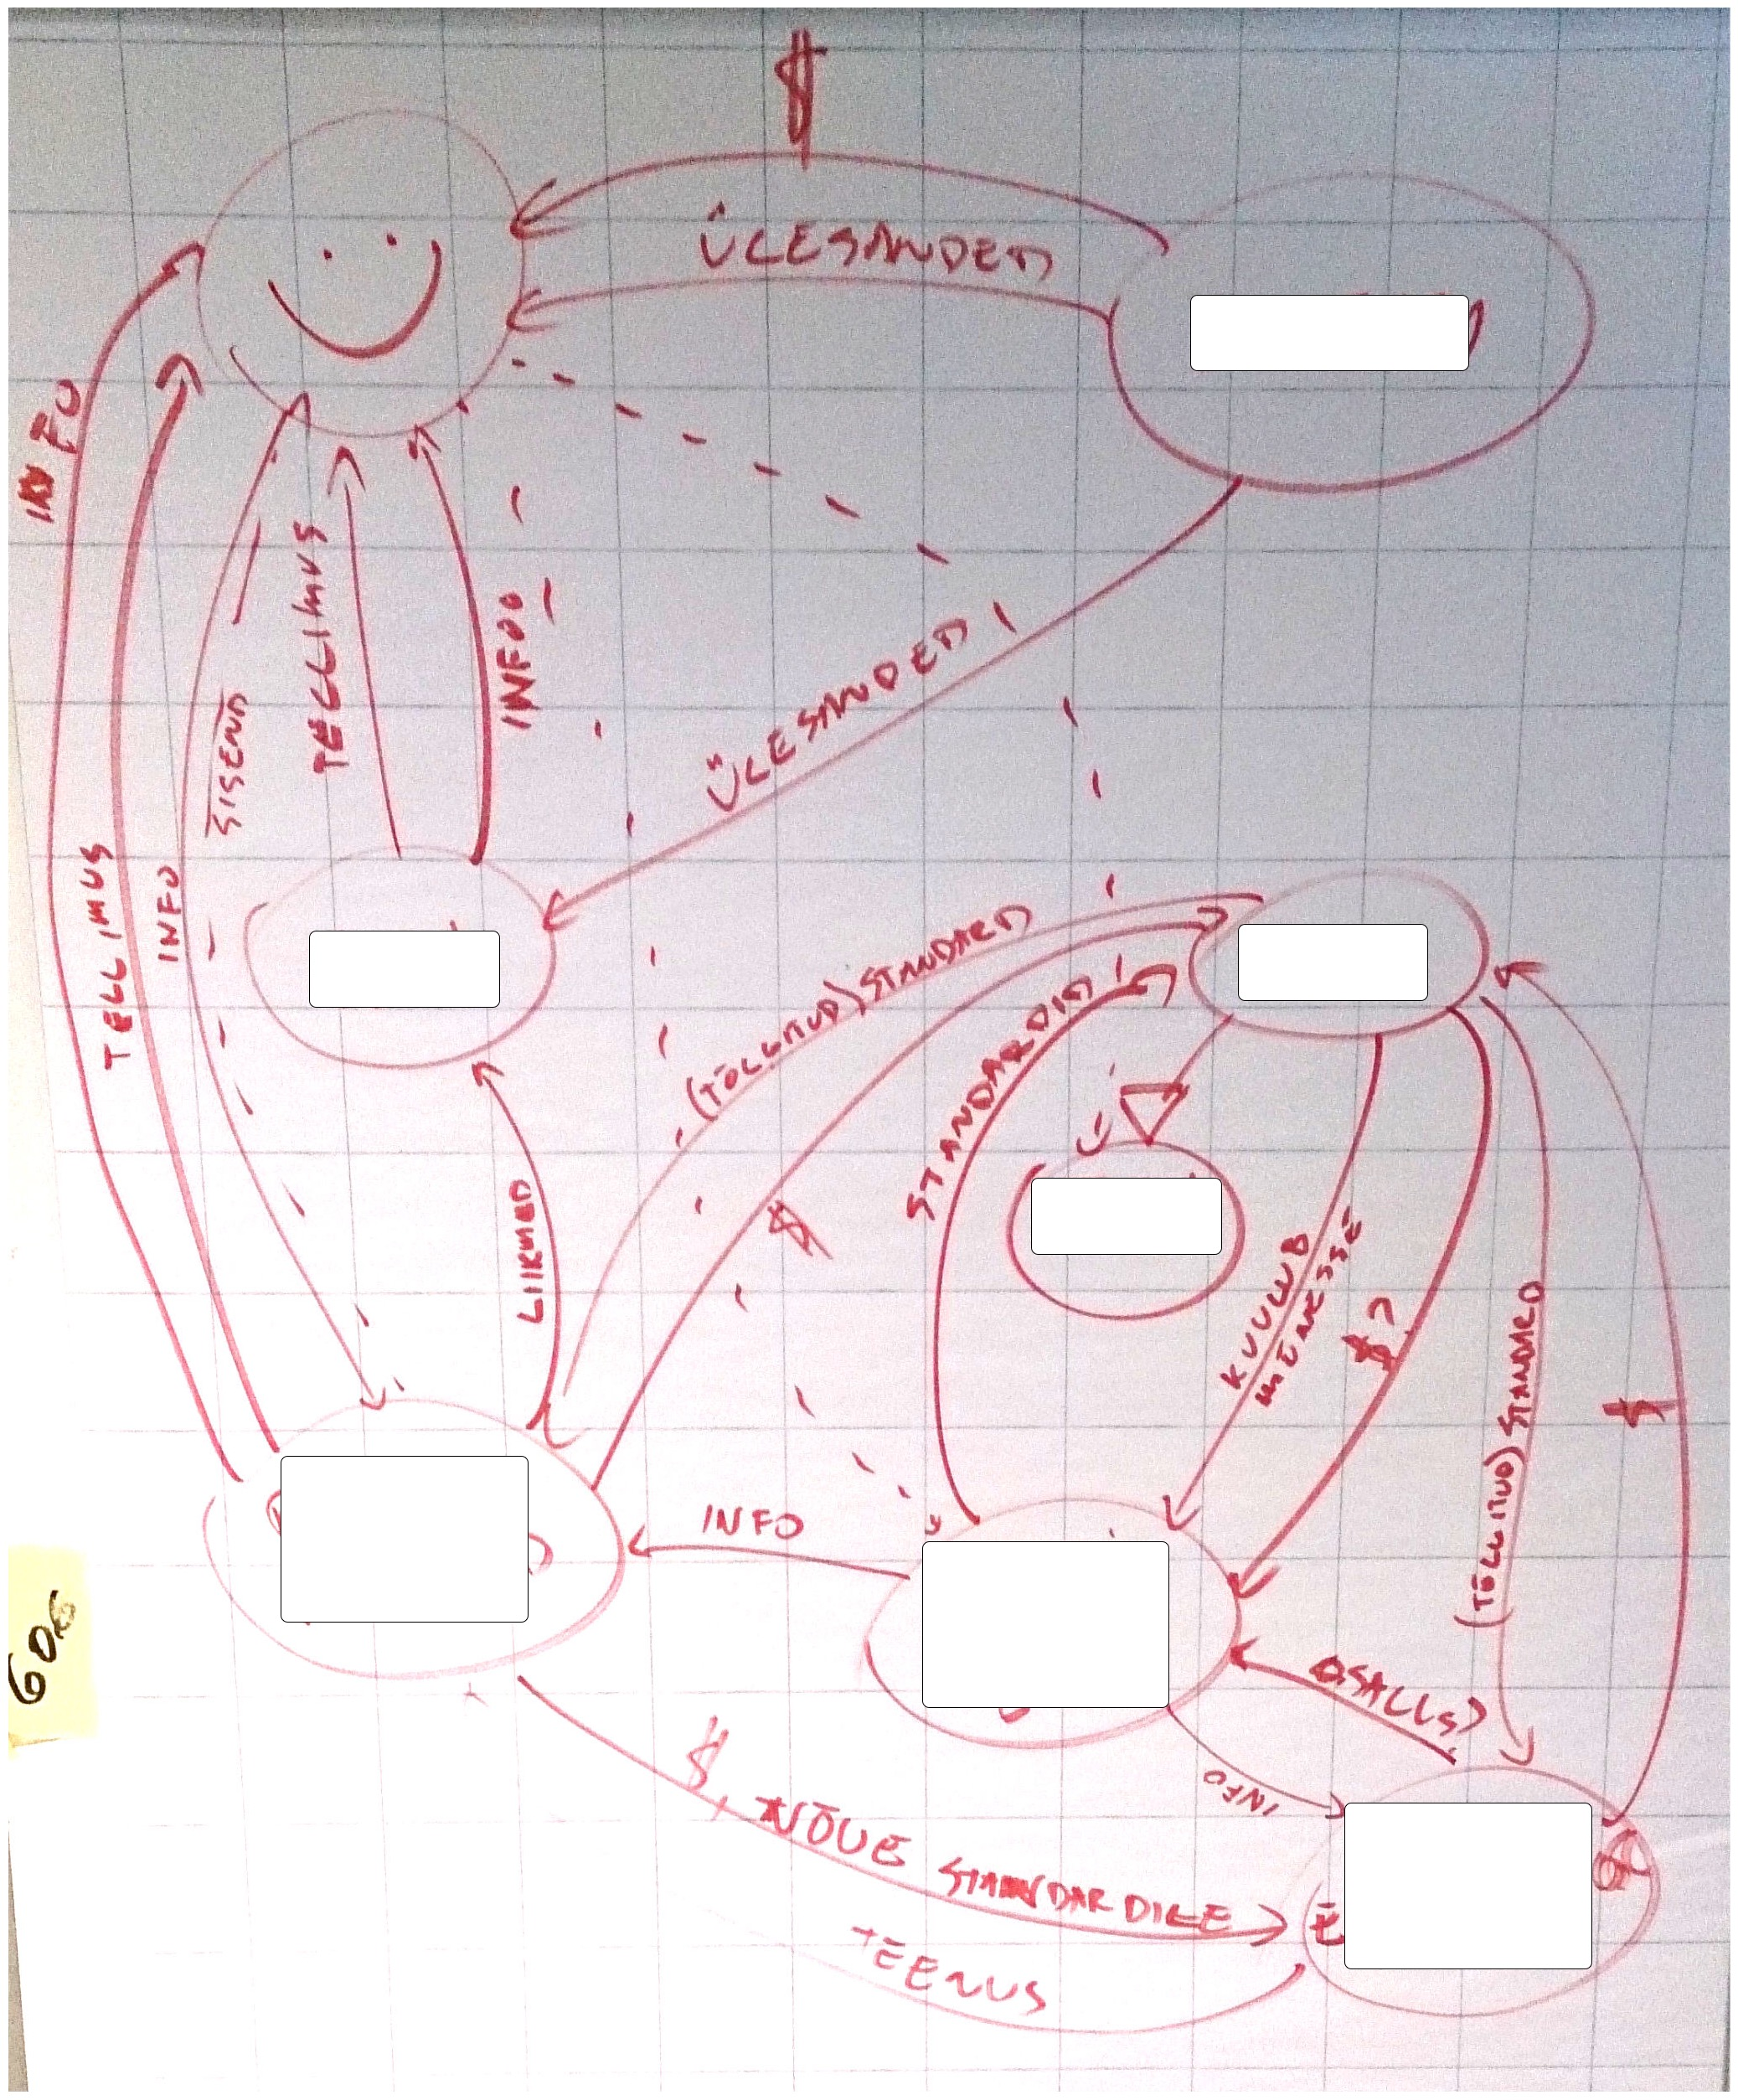
\includegraphics[width=.7\textwidth]{seosed.jpg}
		\caption{Näide seoste diagrammist}
		\label{fig:seosed}
	\end{center}
\end{figure}


\subsection{Piiridest ja nende ületamisest}
Eelmise sajandi seitsmekümnendatel töötas Jay Forrester Rooma Klubi tellimusel välja mudeli maailma rahvastiku kasvu uurimiseks. Forresteri õpilased on mudelit hiljem täiendanud, hetkel on ehk parim lugemismaterial \cite{meadows1992beyond}. Ennustused ei ole roosilised, pigem vastupidi. Ühe tõenäolise võimalusena nähakse ette, et rahavastik ületab suurelt piirid, mida tehnoloogia võimaldab planeedil Maa ära toita ning mahutada ja et järgneb mõõdukas kollaps. Rahvastik kahaneb kiiresti ning palju ning toimub tugev konkurents ressursside pärast (sest kõigile lihtsalt ei jätku). 

\section{Riskijuhtimine}
\subsection{Paradigmamuutus}
Riskijuhtimise paradigmamuutust tingivad järgmised trendid:
	\begin{itemize}
		\item BCP\footnote{\emph{Business Continuity Plan}} keerukus/hind kasvab eksponendina süsteemi keerukusest
			\begin{itemize}
		\item Facebookil ei ole kuskil teist andmekeskust igaks juhuks jõude seismas. See oleks liiga kallis
		\item Väliste partnerite puhul ei ole alati võimalik alternatiivi leida
		\item Äriprotsesside toimimisele ei ole vahel enam mitte-elektroonilist alternatiivi
	\end{itemize}

		\item BCP efektiivsus kahaneb eksponendina süsteemi keerukusest
			\begin{itemize}
		\item Kuidas taastub pilveteenusepakkuja täielikust andmekaost?
		\item Keerulist süsteemi ei pruugi õnnestuda ka mitte ajuti taastada, kui palju ka ei kulutaks. Kui Skype p2p võrk päriselt maha kukub, seda sisuliselt ei olnud võimalik taastada
		\item Äriplaanid, kliendiandmed, ideed, dokumentatsioon on üha enam immateriaalne ja seega kergesti teisaldatav
	\end{itemize}

		\item Üksikute riskisündmuste asemel peame rääkima pidevast, kasvavast ja kuju muutvast survest
			\begin{itemize}
		\item Ka kuritegevuses on edukas see, kes suudab oma ärimudeli võimalikult efektiivselt võimalikult suureks skaleerida
		\item Keerulises süsteemis on väga palju elemente ja nende interaktsioone, mõne katki mineku tõenäosus on suur
		\item Inimese kognitiivset võimet ületavate süsteemide puhul kasvab kiiresti operaatori vigade tõenäosus. Mistõttu ma olen suhteliselt ettevaatlik Eesti Vabariigi infosüsteemi torkimisega
	\end{itemize}

		\item Riskifaktoreid ei saa enam suruda aktsepteeritavale tasemele
			\begin{itemize}
		\item Riik suudab tagada, et tänaval ei jookse nagaaniga vehkiv jõuk, internetis ei ole see võimalik
		\item Süsteemi kõik elemendid ei ole kontrolli all. Vt. esimese kontakti slaidid Yosemite intsidendist
		\item Kuna info liigub, kerkib kiiresti esile uusi (Google: \emph{"ATM gas attacks"})
		\item Turvalist ega vigadeta tarkvara ei ole reaalne toota. Heartbleed istus aastaid laialt kasutatud open source tarkvarateegis kõigi silmade all
	\end{itemize}

\end{itemize}
\subsection{Süsteemiohutuse vaatenurk}
Eelnevalt loetletu kõrvale seab \cite{leveson2011engineering} oma nimekirja asjaoludest, mis sunnivad loobuma senistest süsteemide ohutust käsitlevatest mudelitest:
\begin{itemize}
	\item Kiire tehnoloogiline muutus
	\item Vähenev õppmisvõimekus, mida põhjustab järjest lühenev toote elutsükkel
	\item Õnnetuste iseloom on muutumas, eriti tänu tarkvara tihedasse integreerumisse igapäevaellu
	\item Uued ohtude tüübid. Nanotehnoloogia, keemia, antibiootikumid jne.
	\item Suurenev keerukus ja seotus
	\item Vähenev tolerants üksik-õnnetuste suhtes, mis tuleneb süsteemide suurusest ning meie suurenevast sõltuvusest tehnoloogiast
	\item Prioriteetide seadmise ja valikute tegemise keerukus
	\item Inimeste ja automaatide järjest keerulisemad suhted
	\item Muutuv regulatiivne ja avalikkuse vaade ohutusele. Üksikindiviid ei ole enam suuteline oma vahetu keskkonna ohutust kontrollima
\end{itemize}

\subsection{Kaos ja ahvid}
Üks suurimaid probleeme slaididel ja loengus kirjeldatud paradigmamuutusega toime tulekul on inimeste hoiakud. Kui ühe serveri puhul võis loota, et see niipea katki ei lähe ja kui läheb, siis on teine varuks, siis 1000 serveri puhul läheb iga päev mõni katki. Sama lugu on küberrünnetega. Inimeste mõttemudel muutub aga aeglaselt. Probleemi on huvitavalt lahendanud Netflix \citep{monkey}. Nende vahend lihtsalt käib ja lülitab servereid välja, kõik teavad seda. Ehk, iga teenus peab olema suuteline sellist käitumist taluma. Sisuliselt on Netflix teadmata parameetritega rikete mürafooni asendanud palju tugevama kuid tuntud parameetritega signaaliga.   

\section{Infoturve}
Järgnevas on olulisel määral toetutud Riigi Infosüsteemi Ameti spetsialistide sisendile, mille eest autor on põhjatult tänulik.

\subsection{Korea isikukoodi näide}
2014. aastal tehti Lõuna-Koreas otsus vahetada välja isikukoodid\footnote{Lühike kokkuvõte ja edasisi viiteid saadaval siin \url{https://www.ria.ee/riigiarhitektuur/blog/2014/10/18/south-korea-about-to-overhaul-their-id-card/}}. Põhjuseks asjaolu, et sealne süstem oli üles ehitatud isikukoodi salajasusele. See viimane oli aga disainitud toetuma suhteliselt triviaalsetele turvameetmetele. Tulemuseks oli, et ühest küljest muutus isikukood ahvatlevaks ründeobjektiks ja teisalt olid rea intsidentide tulemusena kümne aasta jooksul sisuliselt kõigi kodanike isikukoodid lekkinud. Ja kuna identiteedivargus on üleüldine, tuleb isikukoodid välja vahetada.

\subsection{Infoturbe strateegiast}
Meid ümbritsevad infosüsteemid on muutunud ülimalt keeruliseks. Seetõttu on sisuliselt võimatuks muutunud toimivate tagavarakoopiate tegemine ja haldamine ning, laiemalt, täielik kontroll süsteemi üle. Samuti on tõsiasi, et kõigist paljudest komponentidest on mõni kogu aeg kas katki või siis ründele haavatav. Lahenduseks tundub olevat terviklik riskikäsitlus, sealhulgas süsteemi turvaliseks disainimine. Kuidas seda aga päriselt ilma kontolli omamata teostada? Head vastust anda ei ole, kui ehk võib abiks olla \cite{leveson2011engineering} ja tema mõtteviis ning arusaam, et keeruliste süsteemide puhul ei saa strateegiliselt eesmärgiks võtta totaalkaitset. Ehk, me ei ürita mitte kõiki süsteemi osa täielikult kontrollida ja kaitsta vaid maandame riskid \emph{piisavale} tasemele jättes teatud riskid teadlikult üles. Sedalaadi lähenemine eeldab aga ülevaadet süsteemi osadest\footnote{Jälle kord kerkib küsimus süsteemi piiridest: kust alates võib riskid ja/või nende maandamise võimekuse lugeda piisavalt väikeseks?}, nende olulisusest süsteemi jaoks ning nende nõrkustest. Õnneks on tegemist riskijuhtimise aabitsatõdedega, vastav teadmine on olemas nii kirjanduses kui praktikas. 

Väga suurel määral sõltub infoturbega tegelemine infost (vt. \ref{sec:valemid}). Järelikult on strateegiliselt oluline tegeleda riskide seirega. Ühest küljest tuleb jälgida oma süsteeme kuid vähemalt sama oluline on pidada silmas lähiümbruses (mis interneti mõistes ei tähenda loomulikult geograafilist lähedust) toimuvat. Siin on olulisel kohal mittetehniline seire: valdkonna kas avalikult või muul moel saada olev info tuleb pidevalt ohuhinnangute uuendamiseks ja prognooside tegemiseks läbi töötada. 

Võib mõelda nii. Kui kõrge on piisavalt kõrge müür sõltub sellest, kui tihti patrull müüri kontrollib ning milline on nende võimekus reageerida. Samuti võib endale madalamaid müüre lubada juhul, kui skaudid ümbrusel silma peal hoiavad ning juba aegsasti pahalaste manöövreid märkavad. 

\subsection{Kuvandi olulisus infoturbes}
Nii valemi \ref{eq:tasuvus} (vt. lk \pageref{eq:tasuvus}) kui teiste riskimudelite puhul on olulisel kohal hinnangulisus. Ründajal on võimalik hinnata kohtuniku käitumist, õiguskaitse tõhusust ning kaitse taga asuva väärtust. Kuid tal ei ole võimalik neid teada. Järelikult on olulisel kohal infoturbes valemi parameetritest ebasoodsa mulje jätmine. Bütsantsi riik kasutas sama taktikat juba aastatuhandete eest, see toimib ka täna. Piltlikult öeldes võib seif olla valmistatud papist, kuid kuni kui kõik usuvad ta olevat läbimatust terasest, keegi talle kääridega ei lähene. Loomulikult on mulje ajutine ning raskesti juhitav ning seetõttu tuleb valmis olla selle purunemiseks. Kui levib info papist seifist, on maailmas kääre küllaga. Samuti ei ole ilmselt mõistlik tekitada kõrge väärtusega sihtmärgi kuvandit lisades ründest oodatavale kasule "feimi" komponendi. 

Jättes kõrvale pideva automatiseeritud ründevoo, võetakse järgmised sihtmärgid kõige tõenäolisemalt ette:
\begin{itemize}
	\item Ettevõtted, millede ründamine on moraalselt õigustatav, mis kuuluvad \emph{fair game} kategooriasse
	\item Ettevõtted, millede kohta on alust arvata, et küberrünne võib teha märkimisväärset kahju
	\item Ettevõtted, millede ründamisel võib olla laiemaid tagajärgi väljaspool sihtmärki
\end{itemize}

\subsection{Rünnete tõsidus}
Eri liiki ründed võib tõsiduse järgi jagada neljaks tasemeks, iga järgnev on eelmisest tõsisem

\begin{enumerate}
	\item Käitlustõrge (näiteks (D)DoS\footnote{\emph{(Distributed) Denial of Service} on rünne, mille käigus ülekoormatakse tahtlikult teenust pakkuv taristu kas ühesest või hajutatud allikast}. Samas on tegemist kõige kõrgema profiiliga ründega, sest paistab lihtsasti välja. Kui teenus puudub, on see kohe kõigile näha
	\item Teenuste ja äritegevuse toimimine mittesoovitud moel. Näiteks Stuxnet, mis ei seisanud rünnatavaid seadmeid, vaid muutis nende tööre\v{z}iimi ning kuvas juhtimismoodulile ebakorrektset infot. Samasse kategooriasse kuulub rünne haigla infosüsteemi vastu millega muudetakse haigete diagnoose, veregruppe jne. 
	\item Teenuse ja äritegevuse usaldusväärsuse langetamine. Kui teenuse usaldusväärsus langeb alla kriitilise piiri, teenust ei kasutata. Seejuures ei ole oluline, kas ja mil määral andmete terviklus või konfidentsiaalsus tegelikult ohus on. Eesti e-riik on selles osas suurepäraseks näiteks: meie riigi toimimine sõltub suurel määral usaldusest terve e-ökosüsteemi (riiklikud institutsioonid, pangad, id-kaart, tehnilised lahendused jne) vastu 
	\item Kontrolli kaotamine teenuse või äritegevuse üle. Sel puhul võetakse üle andmed, kaob kontroll äriprotsesside toimimise üle, teenuste käideldavus kõigub jne.
\end{enumerate}

Arusaam rünnete tõsidusastmest on oluline eriti tänases pidevate rünnete kontekstis. Kuna keegi kogu aeg ründab on oluline keskendada ressursid tegelemaks kõrgema taseme rünnetega. Madalama taseme ründeid võib kas lihtsalt ignoreerida (kui oluline ikkagi on asutuse veebilehe kadumine internetist?) või rahuldaval määral automatiseerimise abil kontrolli alla võttes näiteks paigutades niigi avaliku veebilehe mõne teenusepakkuja elastsesse pilve.

\subsection{Infoturbe valemid} 
\label{sec:valemid}
\subsubsection{Ründe tasuvus}
\begin{equation}
		S_p>P_f(S_a + P_c S_c)
		\label{eq:tasuvus}
\end{equation}

	\begin{description}
		\item[$S_p$] Ründest oodatav kasu
		\item[$P_f$] Ründe ebaõnnestumise tõenäosus
		\item[$S_a$] Ründe läbi viimise kulu
		\item[$P_c$] Vahele jäämise tõenäosus
		\item[$S_c$] Vahele jäämise kulu
	\end{description}

Toodud valemi puhul on oluline silmas pidada kahte asjaolu. 

Esiteks, et ründe ebaõnnestumise tõenäosus on reaalselt alati väiksem kui üks. Põhjuseks lihtsalt sotsiotehniliste süsteemide ülikeerukas olemus. Sihitud ja hoolikalt kavandatud ründe puhul ei ole küsimus selles, kas kaitsest suudetakse läbi murda. Küsimus on selleks kuluvas ajas ja ressursis ning läbimurde sügavuses. Silmas tuleb pidada ka ründevektori "ülevoolavust": alati valitakse ründeks kõige madalama kulu/tulu suhtega vektor. Süsteemide turvalisuse tõstmisega teatud piirist edasi suureneb lihtsalt sotsiaalrünnete surve ning süsteemi kui terviku turvalisus ei tõuse. 

Teiseks, muutujad on alati hinnangulised, neid ei ole ründajal võimalik otseselt mõõta. Siit tuleneb vajadus mõista ründajaid. Tegu on ju lõpuks nende poolt antud hinnangutega. Et eri osapoolte suhtelised võimekused ja huvid on erinevad, on erinevad ka nende hinnangud kulule ning ründest oodatavale kasule. On ju vahe, kas ründajaks on grupp internetiotsingut valdavaid teismelisi või mõne riigi APT\footnote{\emph{Advanced Persistent Threat} on varjatud ja pideva kübersurve oht, mis on suunatud konkreetse ospoole vastu} spetsialistid. 

Kuna evolutsioon dikteerib kõigi osapoolte huvi maksimeerida kasu minimeerides kahju võimaldab ründe tasuvuse analüüs hinnata kõige tõenäolisemaid sihtmärke ning seega planeerida kaitset: kuhu ja kui kõrged müürid ehitada. 

\subsubsection{Riski hinnang}

\begin{equation}
	RISK = Threat \times Consequence \times Vulnerabilities
	\label{eq:risk}
\end{equation}

\begin{description}
	\item[RISK] hinnang riskile
	\item[Threat] hinnang ohule
	\item[Consequence] hinnang riski ohu realiseerumise tagajärgedele
	\item[Vulnerabilities] hinnang süsteemi haavatavusele
\end{description}

Valem \ref{eq:risk} ütleb, et risk on mittelineaarses sõltuvuses ohust, selle realiseerumise tõenäosusest ning süsteemi haavatavusest. Ehk, madala tõenäosuse kuid suure mõjuga oht, millele ollakse haavatavad on sama oluline kui kõrge tõenäosuse ja suure mõjuga oht, mille vastu ollakse hästi kaitstud. Samuti nähtub siit, et iga elemendi nulli viimine viib nulli ka riski. 

Nagu ka valemi \ref{eq:tasuvus} puhul, on siin tegu hinnangutega. Kuid erinevalt ründe tasuvusest on siin ebatäpne mulje pigem probleem, kui lahendus. Kui, eelnevalt kasutatud analoogiat jätkates, seif on papist, on seda kasulik teada ning mitte uskuda teda terasest olevat. Vastasel juhul on oht haavatavust alahinnata. Sama kehtib ka tagajärgede ja ohu kohta. Järelikult on täpne ning teadmistepõhine teadmine olukorrast adekvaatse riskijuhtimise puhul ülioluline.

Absoluutskaalade asemel võib valemi muutujate hindamisel kasutada suhtelisi. Näiteks võib toimida nii:

\begin{enumerate}
	\item Loetle ohud
	\item Anna igale ohule ohuhinnang skaalal 1-10
	\item Anna igale ohule sama skaalat kasutades tagajärje hinnang. Seejuures kata kinni ohuhinnang tagamaks muutujate sõltumatus
	\item Anna igale ohule haavatavushinnang kasutades jällegi sama skaalat ja kattes teised hinnangud kinni
\end{enumerate}

Nüüd oled igale ohule saanud suhtelise riskihinnangu, mis võimaldab neid sorteerida, valida maandamiseks jne.  

\subsubsection{Oodatav kahju} 

	\begin{align}
		Annualised\ Expected\ Loss &= Frequency\ of\ a\ given\ attack\ type \label{eq:loss}\\
		&\times Potential\ Loss \nonumber \\
		&\times Extent\ to\ which\ the\ loss\ occurs \nonumber
	\end{align}

\begin{description}
	\item[Annualised Expected Loss] Oodatav aastane kahju
	\item[Frequency of a given attack type] Konkreetset liiki ründe esinemissagedus
	\item[Potential loss] Potentsiaalne kahju ründest
	\item[Extent to which the loss occurs] Potentsiaalne kahju keskmine realiseerumise määr
\end{description}

Valem \ref{eq:loss} võimaldab hinnata oodatavat kahju ründest. Teades, kui tihti ründed esinevad\footnote{Rünnete esinemise jaotus ning selle hindamine sisuliselt pidevate rünnete tingimustes on keeruline valdkond, millesse siinkohal liigne süveneda}, mis on neist tekkida võiv kahju ning mil määral kahju tavaliselt realiseerub, võib hinnata tekkivat kogukahju. Näiteks, kui meil on keskmiselt kaks tõsisemat teenustõrkerünnet aastas, mis kumbki võivad tekitada 10 000.- \euro kahju ning eelnev kogemus võimaldab hinnata, et kümmekond protsenti kahju õnnestub ära hoida on oodatav kahju $E(L)=2 \times 10000 \times .9 = 18 000$. 

Tegu ei ole infoturbespetsiifilise valemiga, täpselt samuti hinnatakse näiteks krediidiriske.

\section{Juhtimine}
\subsection{Partnerite juhtimine}
Enne, kui asuda end lahutamatult sisse söönud partnerist, "puugist", lahutama, on kasulik veidi mõelda. Asi võib olla selles, et koostöö võib parasiitluse asemel siiski sümbioosiks osutuda. 

On hea teha järgnevat:
\begin{itemize}
	\item Vii kas ise läbi või telli audit hindamaks süsteemi kvaliteeti ning strateegilist positsiooni. Hinnata tuleks nii koodi kui sellist, arhitektuurset lahendust kui ka süsteemi üldist avatust (dokumentatsiooni tase, APIde olemasolu jne.). Audit on kasulik ka sõltumatu argumendina põhjendamaks potentsiaalselt kõrgeid kulusid, mis süsteemide ümber kirjutamise või asendamisega paratamatult kaasnevad (vt. ka \ref{sec:rooste})
	\item Hinda alternatiive. "Puugist" lahti saamine ei ole väga mõistlik, kui järgmisel hankel jälle vaid seesama ettevõte tõsiseltvõetava pakkumise suudab esitada  
\end{itemize}

\subsection{Kvaliteedi juhtimine}
Kuna süsteemide puhul on reeglina tegemist sotsiotehniliste süsteemidega (st. süsteemi osaks loetakse ka lõppkasutaja) on oluliseks süsteemi kvaliteedi parameetriks nende kahe osise omavahaeline koostöö. Samuti väljendub süsteemi kasulikkus reeglina läbi lõppkasutaja. Järelikult on kasutajamugavus ja -kogemus kvaliteedijuhtimise olulised objektid. Reeglina toimub kasutajakogmuse disain süsteemi loomise algfaasis ning kvaliteedi tagamine selle lõpus, mistõttu kaks kompetentsi, paraku, reeglina kokku ei puutu.  

\subsection{Teenustaseme juhtimine}
Tavaliselt on organisatsioonides diskussiooni objektiks teenuse mõiste. Kuna kirjandusest samuti sobilikku määratlust võtta ei ole, siis võivad vaidlused osutuda pikkadeks ja viljatuteks. Seetõttu on oluline välja tuua teenuse definitsiooni kaks peamist struktuurset omadust lisaks slaididel kirjeldatud funktsionaalsetele omadustele:
\begin{itemize}
	\item Definitsioon peab suutma tõmmata selge, organisatsiooni ülevalt alla läbiva, piiri eri teenuste vahele
	\item Definitsioon peab olema vastuvõetav tervele organisatsioonile
\end{itemize}

samas:
\begin{itemize}
	\item Definitsioon ei pea olema täielik, määratletavad teenused ei pea katma kõiki organisatsiooni tegevusvaldkondi
	\item Definitsioon võib olla meelevaldne ("Teenuseks on rakendusse sisse logimine ja meie töötajate füüsiline kohalolu leti taga, miski muu teenus ei ole")
\end{itemize}

Kui esimesed kaks tingimust on täidetavad, võib vaidlused lõppenuks lugeda ning asuda teenustaset jutima.




\nocite{*}
\bibliographystyle{plainnat}
\bibliography{it_strateegia} 

\end{document}
